% !TeX spellcheck = <none>
\documentclass[11pt]{charter}
\usepackage[shortlabels]{enumitem}
\usepackage{enumitem}
\usepackage{pdflscape}
\usepackage[official]{eurosym}
\usepackage{afterpage}
\usepackage{lipsum}


% El títulos de la memoria, se usa en la carátula y se puede usar el cualquier lugar del documento con el comando \ttitle
\titulo{Sistema de sensores autónomos para monitoreo de redes de distribución de baja tensión mediante LoRaWAN} 

% Nombre del posgrado, se usa en la carátula y se puede usar el cualquier lugar del documento con el comando \degreename
\posgrado{Carrera de Especialización en Sistemas Embebidos} 
%\posgrado{Carrera de Especialización en Internet de las Cosas} 
%\posgrado{Carrera de Especialización en Intelegencia Artificial}
%\posgrado{Maestría en Sistemas Embebidos} 
%\posgrado{Maestría en Internet de las cosas}

% Tu nombre, se puede usar el cualquier lugar del documento con el comando \authorname
\autor{Ing. Milton Eduardo Sosa} 

% El nombre del director y co-director, se puede usar el cualquier lugar del documento con el comando \supname y \cosupname y \pertesupname y \pertecosupname
\director{Ing. Marcelo E. Romeo}
\pertenenciaDirector{UNSAM} 
% FIXME:NO IMPLEMENTADO EL CODIRECTOR ni su pertenencia
\codirector{} % si queda vacio no se deberíá incluir 
\pertenenciaCoDirector{}

% Nombre del cliente, quien va a aprobar los resultados del proyecto, se puede usar con el comando \clientename y \empclientename
\cliente{Ing. Marcelo E. Romeo}
\empresaCliente{Universidad Nacional de San Martín}

% Nombre y pertenencia de los jurados, se pueden usar el cualquier lugar del documento con el comando \jurunoname, \jurdosname y \jurtresname y \perteunoname, \pertedosname y \pertetresname.
\juradoUno{Nombre y Apellido (1)}
\pertenenciaJurUno{pertenencia (1)} 
\juradoDos{Nombre y Apellido (2)}
\pertenenciaJurDos{pertenencia (2)}
\juradoTres{Nombre y Apellido (3)}
\pertenenciaJurTres{pertenencia (3)}
 
\fechaINICIO{22 de junio de 2020}		%Fecha de inicio de la cursada de GdP \fechaInicioName
\fechaFINALPlanificacion{22 de Agosto de 2020} 	%Fecha de final de cursada de GdP
\fechaFINALTrabajo{22 de Diciembre de 2020}		%Fecha de defensa pública del trabajo final


\begin{document}

\maketitle
\thispagestyle{empty}
\pagebreak


\thispagestyle{empty}
{\setlength{\parskip}{0pt}
\tableofcontents{}
}
\pagebreak


\section{Registros de cambios}
\label{sec:registro}


\begin{table}[ht]
\label{tab:registro}
\centering

\begin{tabularx}{\linewidth}{@{}|c|X|c|@{}}
\hline
\rowcolor[HTML]{C0C0C0} 
Revisión & \multicolumn{1}{c|}{\cellcolor[HTML]{C0C0C0}Detalles de los cambios realizados} & Fecha      \\ \hline
1.0      & Creación del documento                                                          & 22/06/2020 \\ \hline
1.2      & Avances hasta el desglose de trabajo en tareas.                                 & 10/07/2020 \\ \hline
1.3      & Se corrigen errores ortográficos y espaciado entre párrafos. \newline
	Se agranda el tamaño de las figuras 1 y 2.\newline
	Marcelo E. Romeo pasa a ocupar el rol de cliente.\newline
	Se corrigen los requerimientos y estimaciones del desglose del trabajo en tareas.\newline
	Se agregan tareas de documentación
%\shortstack[l]{}
& 17/07/2020 \\ \hline

1.4      & Se desarrollan los puntos 6 al 11.\newline
	Se modifica el valor del presupuesto en base a la cotización del día del Banco Central de la República Argentina.\newline
& 31/07/2020 \\ \hline
1.5      & Se desarrollan los puntos 12 al 17                                                  & 08/08/2020 \\ \hline
\end{tabularx}
\end{table}

\pagebreak



\section{Acta de Constitución del Proyecto}
\label{sec:acta}

\begin{flushright}
Buenos Aires, \fechaInicioName
\end{flushright}

\vspace{2cm}

Por medio de la presente se acuerda con el \authorname\hspace{1px} que su Trabajo Final de la \degreename\hspace{1px} se titulará ``\ttitle'', consistirá esencialmente en el prototipo preliminar de un sistema embebido que sea capaz de determinar valores eficaces de corriente alterna en redes de distribución de baja tensión y enviarlos a un centro de operaciones. Será no invasivo y autónomo. Tendrá un presupuesto preliminar estimado de 676 hs de trabajo y \$887.356, ochocientos ochenta y siete mil trescietos cincuenta y seis pesos argentinos, con fecha de inicio \fechaInicioName\hspace{1px} y fecha de presentación pública \fechaFinalName.

Se adjunta a esta acta la planificación inicial.

\vfill

% Esta parte se construye sola con la información que hayan cargado en el preámbulo del documento y no debe modificarla
\begin{table}[ht]
\centering
\begin{tabular}{ccc}
\begin{tabular}[c]{@{}c@{}}Ariel Lutenberg \\ Director posgrado FIUBA\end{tabular} &  & \begin{tabular}[c]{@{}c@{}}\clientename \\ \empclientename \end{tabular} \vspace{2.5cm} \\ 
\multicolumn{3}{c}{\begin{tabular}[c]{@{}c@{}} \supname \\ Director del Trabajo Final\end{tabular}} \vspace{2.5cm} \\
\begin{tabular}[c]{@{}c@{}}\jurunoname \\ Jurado del Trabajo Final\end{tabular}     &  & \begin{tabular}[c]{@{}c@{}}\jurdosname\\ Jurado del Trabajo Final\end{tabular}  \vspace{2.5cm}  \\
\multicolumn{3}{c}{\begin{tabular}[c]{@{}c@{}} \jurtresname\\ Jurado del Trabajo Final\end{tabular}} \vspace{.5cm}                                                                     
\end{tabular}
\end{table}




\section{Descripción técnica-conceptual del Proyecto}
\label{sec:descripcion}

%\begin{consigna}{black}
El presente trabajo surge como idea del autor, en base a la necesidad de permitir a las redes de distribución metropolitanas y megalopolitanas integrar características de las así llamadas Ciudades Inteligentes y así enmarcarlas dentro del concepto de Internet de las Cosas (IoT). Una ciudad inteligente, es aquella que hace uso de las diferentes tecnologías de información y comunicación disponibles con el objetivo de lograr su desarrollo sostenible, mejorar la calidad de vida de los ciudadanos y hacer un uso eficiente de los recursos energéticos.\\

Se siguen las premisas de minimizar impactos y costos de implementación en las redes de distribución actual y a la vez lograr un aumento en la calidad de servicio de energía eléctrica haciendo uso de los datos relevados.\\

Es menester mencionar que este trabajo es parte de un proyecto de una PyME de base tecnológica con el objeto de prestar servicios a diferentes empresas distribuidoras de energía electrica en Sudamérica, como así también a personas que deseen monitorear el estado de una carga eléctrica en particular haciendo uso de una estructura de red de comunicación de largo alcance.\\

El sistema que se propone implementar, ocuparía un mínimo espacio físico adicional en la red. Sin embargo, la información que proporcionaría sería de gran relevancia para realizar un relevamiento en tiempo semi real del estado de operación de la red de distribución de energía eléctrica.\\

Entre las características técnicas que sobresalen de este sistema se encuentra la utilización de tecnologías de comunicación de largo alcance y bajo consumo de energía, como por ejemplo LoRa y redes LoRaWAN, para reportar el estado de operación de un nodo en particular de la red. También propone el uso de formas de conversión y acumulación de energía eléctrica de bajo impacto medioambiental con el objeto de lograr autonomía de operación aún en condiciones meteorológicas desfavorables y operando en régimen 24/7.\\

Finalmente, es la intención de que este prototipo se mantenga independiente de la frecuencia y tensión de operación otorgando así, facilidad a la hora de realizar el comisionamiento en diferentes redes.\\

El sistema propuesto se compondrá por un hardware (HW) a desarrollar para cada nodo y los servicios interconectados en la nube también llamados backend services (BES).\\
\label{sec:diagrama_de_bloques_HW}\\
El diagrama de bloques del HW a desarrollar es presentado en la Figura \ref{fig:diagBloques}. Este posee cinco etapas:
\vspace{25px}
\begin{figure}[H]
	\centering 
	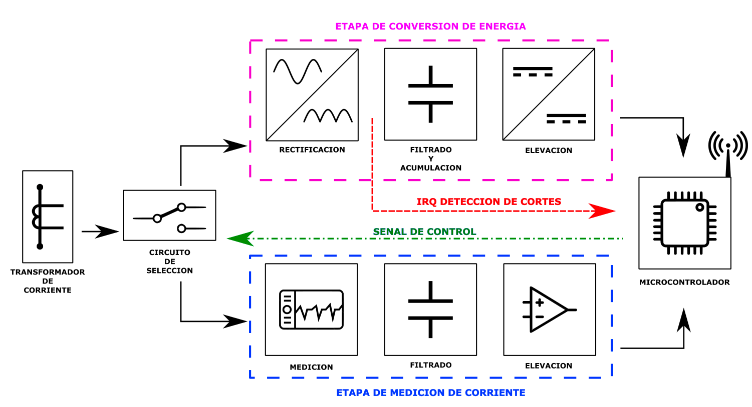
\includegraphics[width=\textwidth]{./Figuras/HW_block_diagram.png}
	\caption{Diagrama en bloques del hardware asociado al sistema.}
	\label{fig:diagBloques}
\end{figure}
\vspace{15px}
\begin{itemize}
	\item Transformador de corriente (TI): encargado de proveer de corriente eléctrica para la carga del acumulador, como así también actuar como  transductor de corriente para la medición de su valor eficaz.\\

	\item Etapa de conversión y acumulación de energía: compuesta por un rectificador de baja caída, un acumulador y un conversor DC/DC.\\

	\item Etapa de medición/detección de corriente: encargado de las mediciones de valor eficaz de corriente alterna junto a un circuito de acondicionamiento de señal.\\

	\item Circuito de selección de modo: compuesto por un relay (RL) acorde al TI y su circuito de excitación.\\

	\item Etapa de procesamiento, control y comunicaciones: compuesto por un microcontrolador (uC) y un módulo de comunicaciones (MC) LoRa.\\
\end{itemize}
Para lograr la recuperación de datos generados por el HW y enviados a la red LoRaWAN, es necesario contar con un conjunto de servicios privados de backend (BES). Estos deberán estar integrados de manera permanente con la red LoRaWAN, que se considera preexistente, y cuya infraestructura es presentada en la Figura \ref{fig:diagBloquesLoRaWAN}.\\

\begin{figure}[H]
	\centering 
	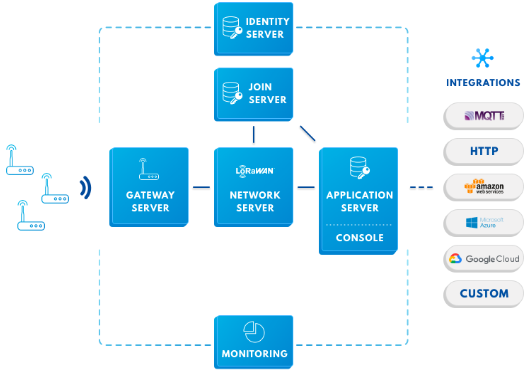
\includegraphics[width=\textwidth]{./Figuras/arquitectura_TTN.png}
	\caption{Diagrama en bloques de la red LoRaWAN a utilizar y sus posibles integraciones con terceras partes.}
	\label{fig:diagBloquesLoRaWAN}
\end{figure}

Esta integración se logrará a través de APIs HTTP o mediante suscripciones a tópicos de agentes de mensajería.\\
Los BES privados a desarrollar en este proyecto serán 3:
\begin{enumerate}
	\item Servicio de Recuperación de Datos: encargado de recuperar los datos enviados por los nodos a traves de la API proporcionada por la red LoRaWAN y almacenarlos en una base de datos.
	\item Base de datos (DB): encargado de almacenar los valores históricos de los nodos sensores y generar diferentes métricas para los reportes de estado.
	\item Interfaz Gráfica de Usuario (GUI): encargada de presentar el último estado recuperado de cada nodo al usuario final del sistema.
\end{enumerate}
%\end{consigna}


\section{Identificación y análisis de los interesados}
\label{sec:interesados}

\begin{consigna}{black} 

\begin{table}[H]
%\caption{Identificación de los interesados}
%\label{tab:interesados}
\begin{tabularx}{\linewidth}{@{}|l|X|X|l|@{}}
\hline
\rowcolor[HTML]{C0C0C0} 
Rol           & Nombre y Apellido & Organización 	& Puesto 	\\ \hline
Cliente    & \supname & \pertesupname & Docente investigador \\ \hline
\shortstack[l]{Responsable, auspiciante \\ e impulsor} & Ing. Milton E. Sosa & Universidad Nacional de Misiones & Egresado\\ \hline
Orientador    & \supname	      & \pertesupname 	& Docente investigador \\ \hline
Colaborador & Dr. Ing. Eduardo O. Sosa  &Universidad Nacional de Misiones &Docente Investigador    	\\ \hline
Colaborador & Ing. Germán A. Xánder     &Universidad Nacional de Misiones &Docente Investigador    	\\ \hline
Usuario final &                   &              	&        	\\ \hline
\end{tabularx}
\end{table}
 
\begin{itemize}
	\item Ing. Marcelo E. Romeo, de vasta experiencia profesional en el ámbito de la microelectrónica e investigación y desarrollo para diferentes entidades y universidades nacionales.
	\item Dr. Ing. Eduardo O. Sosa, cuenta con más de 20 años de experiencia en el área de las TELCO, ex miembro colaborador de la RIU, profesor titular de la cátedra de Física en la Universidad Nacional de Misiones y lidera proyectos bilaterales entre Argentina y Alemania en el ámbito de WSN.
\end{itemize}
\end{consigna}

\section{1. Propósito del proyecto}
\label{sec:proposito}

\begin{consigna}{black}
El propósito de este proyecto es desarrollar un sistema formado por un circuito electrónico autónomo y un conjunto de software dedicado a la recuperación y almacenamiento de datos generados y transmitidos por el circuito.\\

El sistema debe ser capaz de permitir a las actuales redes de distribución de energía eléctrica reportar su estado actual de operación a un centro de monitoreo.
\end{consigna}

\section{2. Alcance del proyecto}
\label{sec:alcance}

\begin{consigna}{black}
Se pretende desarrollar un prototipo de HW capaz de ser autosuficiente en cuanto a la conversión, acumulación y gestión de energía eléctrica con el objeto de alimentar y permitir su operación en estado autónomo y permanente. Para ello se desarrollará un circuito de \textit{micro energy harvesting} basado en rectificadores de bajas pérdidas, acumuladores aptos para la aplicación final y un conversor DC/DC de alta eficiencia.\\

Se desarrollará una etapa de medición de valor eficaz de corriente alterna, con el objeto de medir la intensidad de corriente que actualmente circula por el conductor conectado a la salida de baja tensión e inmediatamente después del fusible aéreo de protección.\\

Agregado a los módulos mencionados anteriormente, un microcontrolador se encargará de la gestión de energía de todo el HW y de digitalizar todas las mediciones realizadas para finalmente, enviarlas al centro de operaciones a través de un módulo de comunicación.\\

Los BES se albergarán en una computadora de bajo costo que proporcionará suficientes recursos para su operación y ensayo en la etapa de desarollo.\\

No es parte del alcance del presente proyecto llegar a una etapa de lanzamiento del producto a clientes finales, sino la de lograr un demostrador tecnológico. Sin embargo, si los tiempos lo permiten y se logra contar con una infraestructura adecuada, se desean realizar ensayos \textit{end-to-end} en laboratorio sobre el sistema, involucrando los prototipos de hardware que fueran desarrollados, y una integración mínima entre los BES y la red LoRaWAN ya existente.\\
\end{consigna}

\section{3. Supuestos del proyecto}
\label{sec:supuestos}
\begin{consigna}{black}
Para el desarrollo del presente proyecto se supone que:
\begin{itemize}
	\item El autor del trabajo no tendrá ningún problema para hacerse de los insumos necesarios para alcanzar los objetivos recurriendo a distribuidores de componentes en el mercado local.
	\item Al momento de ensayar el sistema se contará con conectividad a internet.
	\item El responsable no tendrá en ningún momento limitaciones de movilidad.
	\item En caso de ser necesario realizar ensayos \textit{end-to-end}, el responsable deberá fabricar un banco de ensayos apropiado para simular los casos de uso y probar el sistema en su conjunto, como así disponer de instrumentos patrones para contrastar y verificar el correcto funcionamiento.
	\item Los ensayos \textit{end-to-end} no demorarán la fecha de finalización del proyecto.
\end{itemize}
\end{consigna}





\section{4. Requerimientos}
\label{sec:requerimientos}
%\begin{consigna}{black}
\begin{enumerate}
\item Grupo de requerimientos asociados con hardware
	\begin{enumerate}
	\item El dispositivo deberá ser de tipo \textit{plug and play}.
	\item El circuito impreso no deberá ocupar un volumen mayor a 10x10x5 cm.
	\item Basarse en un microcontrolador ESP32 y disponer de:
	\begin{enumerate}[label*=\arabic*.]
		\item 4 entradas analógicas.
		\item 3 salidas digitales.
		\item Unidad UART.
		\item Integrar un módulo de comunicaciones LoRa.
	\end{enumerate}
	\item Deberá tener al menos 12 horas de autonomía de funcionamiento.
	\item Bajo consumo en modo ocioso: el consumo del hardware en total, no deberá superar los 5 mA cuando no está midiendo ni transmitiendo.
	\item El circuito elevador de tensión DC-DC deberá:
	\begin{enumerate}[label*=\arabic*.]
		\item Funcionar con tensiones menores a 2V en la entrada.
		\item Otorgar 5 Volts a la salida.
		\item Ser capaz de otorgar 300 miliamperes a la salida.
	\end{enumerate}
	\item El transformador de corriente debe:
	\begin{enumerate}[label*=\arabic*.]
		\item Ser de tipo núcleo partido.
		\item Admitir 100 Amperes de corriente en el circuito primario y un máximo 5 Amperes en el circuito secundario.
	\end{enumerate}
	\item \label{req_relay} El relay encargado de cambiar el modo de operación debe:
	\begin{enumerate}[label*=\arabic*.]
		\item Ser de tipo doble invesor sin retención.
		\item Su bobina debe poder energizarse con 5V o menos.
		\item Soportar al menos 5 Amperes de corriente por los contactos.
	\end{enumerate} 
	\item Debe funcionar de manera independiente a la frecuencia de operación de la red 50/60 Hz.
	\item Debe funcionar de manera independiente a la tensión de fase del sistema de distribución 110/220 Voltios.
	\end{enumerate}
	
\item Grupo de requerimientos asociados con el firmware
	\begin{enumerate}
	\item Debe manejar un módulo de comunicación LoRa y protocolo LoRaWAN.
	\item Deberá tener un porcentaje de cobertura de tests unitarios del 60\% como mínimo.
	\item Antes configurarse en modo ocioso, debe desenergizar la etapa de medición de corriente y el módulo de comunicaciones con el objeto de ahorrar energía.
	\end{enumerate}
	
\item Grupo de requerimientos asociados con los BES
	\begin{enumerate}
		\item Todos los servicios deben poder correr en una Raspberry Pi 3.
		\item El software de los BES se desarrollará en lenguaje Python.
		\item Recuperar los datos de la red LoRaWAN.
		\item Almacenar los datos en una tabla de MySQL.
		\item GUI basada en Grafana.
	\end{enumerate}

\item Grupo de requerimientos asociados con ensayos de integración y \textit{end-to-end}
	\begin{enumerate}
		\item El banco de ensayos de hardware debe contar con una carga fantasma de al menos 10 Amperes y permitir realizar interrupciones de corriente de manera programada mediante una computadora adicional tipo Raspberry Pi o de manera manual.
		\item Los BES deben estar operativos al momento de realizar los ensayos.
		\item Contar con un gateway de acceso a una red LoRaWAN como por ejemplo \textit{The Things Network}.
	\end{enumerate}
\end{enumerate}
%\end{consigna}

\section{Historias de usuarios (\textit{Product backlog})}
\label{sec:backlog}

\section{5. Entregables principales del proyecto}
\label{sec:entregables}
%\begin{consigna}{black}
\begin{itemize}
\item Diagrama esquemático
\item Lista de materiales
\item Código fuente del firmware
\item Diagrama de instalación
\item Informe final
\end{itemize}

%\end{consigna}

\section{6. Desglose del trabajo en tareas}
\label{sec:wbs}
%\begin{consigna}{black}
\begin{enumerate}
\item Grupo de tareas asociadas a planificación (Total: 35 hs)
	\begin{enumerate}
		\item Diseño de la arquitectura global del proyecto. (15 hs)
		\item Documentación del plan de proyecto. (20 hs)
	\end{enumerate}
\item Grupo de tareas asociadas al hardware (Total: 300 hs)
	\begin{enumerate}
		 \item Transductor de corriente. (Total: 16 hs)
			 \begin{enumerate}[label*=\arabic*.]
			 	\item Análisis de transductores aptos para el hardware a desarrollar. (5 hs)
			 	\item Selección de componentes. (3 hs)
			 	\item Ensayo y evaluación del transductor de manera individual. (4 hs)
			 	\item Documentación de resultados del ensayo del transductor. (4 hs)
			 \end{enumerate}
			
		 \item Etapa de circuito de selección. (Total: 24 hs)
			 \begin{enumerate}[label*=\arabic*.]
			 	\item Análisis de alternativas disponibles en el mercado. (10 hs)
			 	\item Selección de relays aptos en base a los requerimientos: tensión de bobina de 5 Volts y 5 Amperes de corriente. (6 hs)
			 	\item Ensayo del circuito de selección de manera individual. (4 hs)
			 	\item Documentación de ensayo. (4 hs)
			 \end{enumerate}			
			
		 \item Etapa de rectificación y filtrado. (Total: 49 hs)
			 \begin{enumerate}[label*=\arabic*.]
				\item Análisis comparativo de alternativas para técnicas de rectificacion. (30 hs)
				\item Selección de componentes encargados de la etapa de rectificación. (10 hs)
				\item Ensayo de la etapa de rectificación de manera individual. (5 hs)
				\item Documentación de ensayos. (4 hs)
			 \end{enumerate}
			
		 \item Etapa de acumulación de energía. (Total: 35 hs)
			 \begin{enumerate}[label*=\arabic*.]
			 	\item Análisis comparativo y selección de alternativas viables acorde al requerimiento de autonomía de operación. (10 hs)
			 	\item Ensayo de carga y descarga del acumulador de manera individual. (10 hs)
			 	\item Evaluación de resultados y estimación de la autonomía de operación en función de diferentes perfiles de consumo. (10 hs)
			 	\item Documentación ensayos. (5 hs)
			 \end{enumerate}
			 
		 \item Etapa de elevación de tensión. (Total: 20 hs)
			 \begin{enumerate}[label*=\arabic*.]
			 	\item Análisis de alternativas técnicas para elevación de tensión aptas para el hardware a desarrollar. (15 hs)
			 	\item Ensayo y evaluación de la etapa de elevación de tensión de manera individual. (5 hs)
			 \end{enumerate}

		 \item Etapa de medición de corriente. (Total: 34 hs)
			 \begin{enumerate}[label*=\arabic*.]
			 	\item Análisis comparativo y selección de un ciruito integrado dedicado a realizar la medición del valor eficaz de corriente. (20 hs)
			 	\item Ensayo y evaluación de la etapa de medición de valor eficaz de manera individual. (10 hs)
			 	\item Documentación de ensayos. (4 hs)
			 \end{enumerate}
			 
		 \item Etapa de acondicionamiento de señal posterior a la medición de corriente. (Total: 13 hs)
			 \begin{enumerate}[label*=\arabic*.]
			 	\item Análisis de alternativas técnicas para filtrado y amplificación. (4 hs)
			 	\item Selección de componentes. (2 hs)
			 	\item Ensayo y evaluación de la etapa de filtrado y amplificación de manera individual. (4 hs)
			 	\item Documentación de ensayos. (3 hs)
			 \end{enumerate}
			 
		 \item Microcontrolador y módulo de comunicaciones. (Total: 50 hs)
			 \begin{enumerate}[label*=\arabic*.]
			 	\item Análisis y selección de microcontroladores y módulos de comunicaciónes aptos para la aplicación. (30 hs)
			 	\item Pruebas de laboratorio del microcontrolador y módulo de comunicaciónes de manera individual. (20 hs)
			 \end{enumerate}
		
		 \item Circuito impreso. (Total: 59 hs)
			 \begin{enumerate}[label*=\arabic*.]
			 	\item Ruteo del circuito impreso. (40 hs)
			 	\item Inspección. (6 hs)
			 	\item Montaje y soldado de componentes. (8 hs)
			 	\item Prueba y depuración. (5 hs)
			 \end{enumerate}			 			 			 
		\end{enumerate}

	\item Grupo de tareas asociadas al software (Total: 206 hs)
	\begin{enumerate}
		\item Tareas asociadas al firmware del microcontrolador (Total: 110 hs)
			\begin{enumerate}[label*=\arabic*.]
				\item Definición de la "lógica de negocio" que regirá la operación del hardware a instalar \textit{in-situ}. (10 hs)
				\item Prototipado del firmware. (60 hs)
				\item Depuración de errores. (20 hs)
				\item Pruebas unitarias. (20 hs)
			\end{enumerate}
		
		 \item Tareas asociadas a los BES (Total: 96 hs)
			\begin{enumerate}[label*=\arabic*.]
				\item Diseño de la arquitectura y lógica de operación de cada servicio. (14 hs)
				\item Instalación de los servicios. (30 hs)
				\item Creación de tablas en base de datos para el almacenamiento de valores históricos. (4 hs)
				\item Desarrollo del software encargado de recuperar los datos de la red LoRaWAN y almacenar en la base de datos. (20 hs)
				\item Desarrollo de la interfaz gráfica en Grafana. (8 hs)
				\item Pruebas de integración. (15 hs)
				\item Depuración de errores. (5 hs)
			\end{enumerate}
		\end{enumerate}
		
	\item Grupo de tareas asociadas a pruebas \textit{end-to-end}. (Total: 65 hs)
		\begin{enumerate}
		 	\item Definición de los casos de ensayo. (20 hs)
		 	\item Desarrollo del software. (20 hs)
		 	\item Ejecución de las pruebas. (15 hs)
		 	\item Depuración de errores. (10 hs)
		\end{enumerate}		

	\item Grupo de tareas asociadas al cierre del proyecto (Total: 70 hs)
		\begin{enumerate}
			\item Elaboración de la memoria técnica. (50 hs)
			\item Elaboración de la presentación final. (20 hs)
		\end{enumerate}
	\end{enumerate}
	
Cantidad total de horas: (676 hs)

%\end{consigna}

\section{7. Diagrama de Activity On Node}
\label{sec:AoN}
\begin{figure}[htpb]
	\centering 
	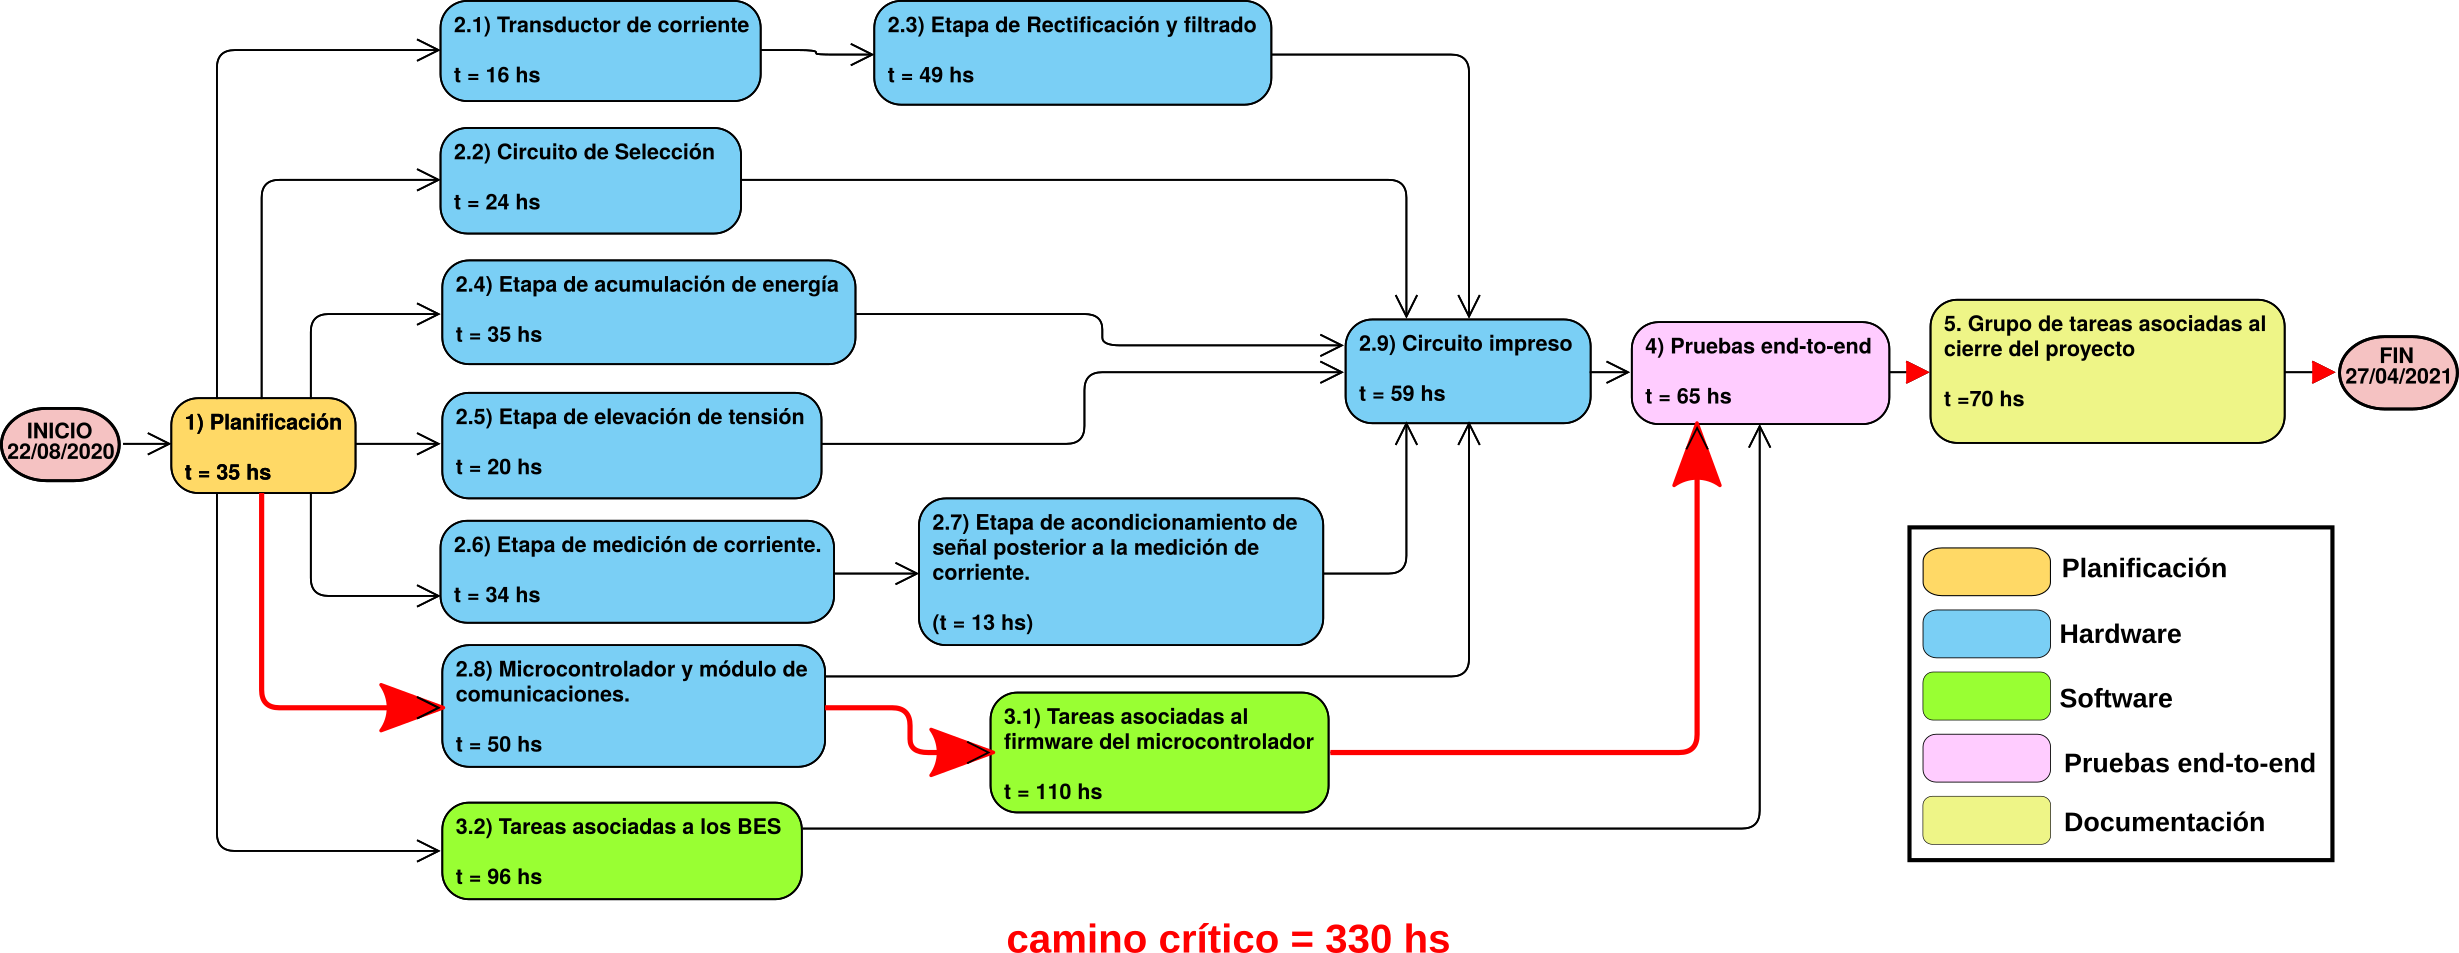
\includegraphics[width=\textwidth]{./Figuras/activity_on_node/version_compacta/aon.png}
	\caption{Diagrama en \textit{Activity on Node}}
	\label{fig:AoN}
\end{figure}


\section{8. Diagrama de Gantt}
\label{sec:gantt}
\begin{figure}[H]
	\centering 
	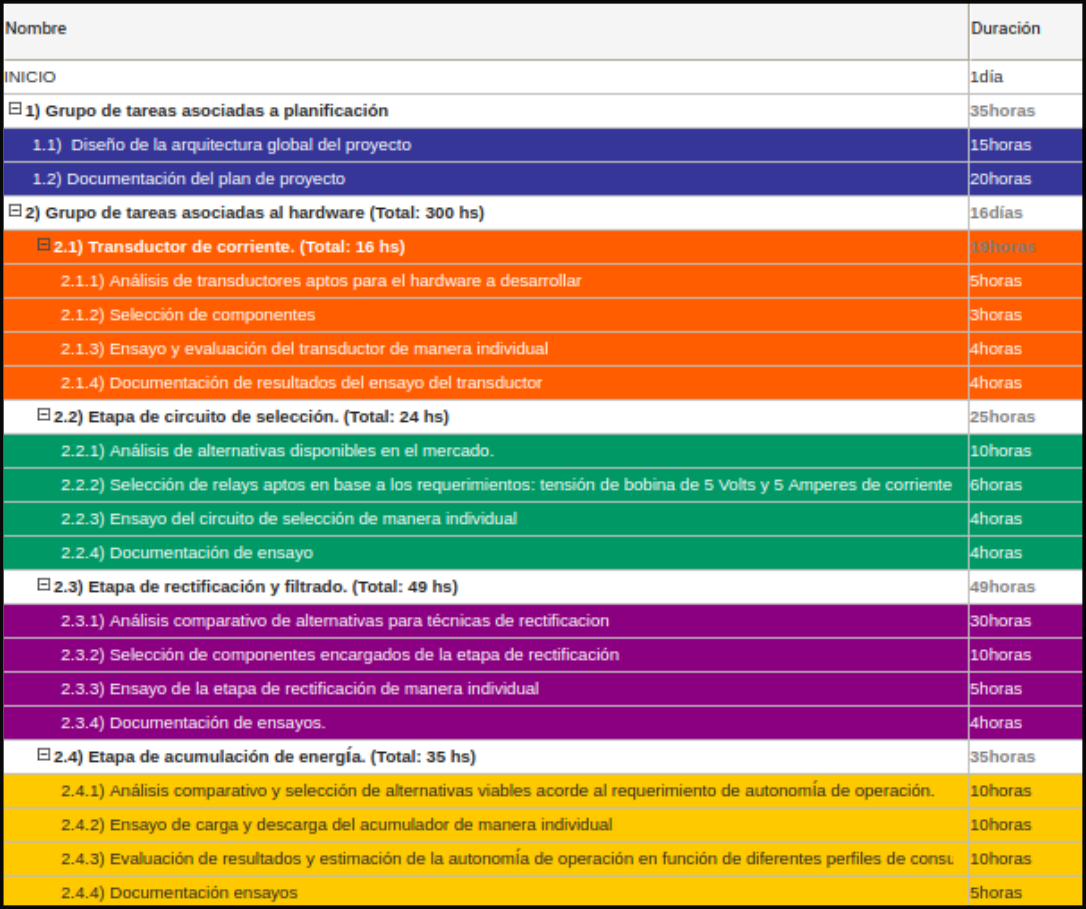
\includegraphics[width=\textwidth]{./Figuras/gantt/inicio-24.png}
	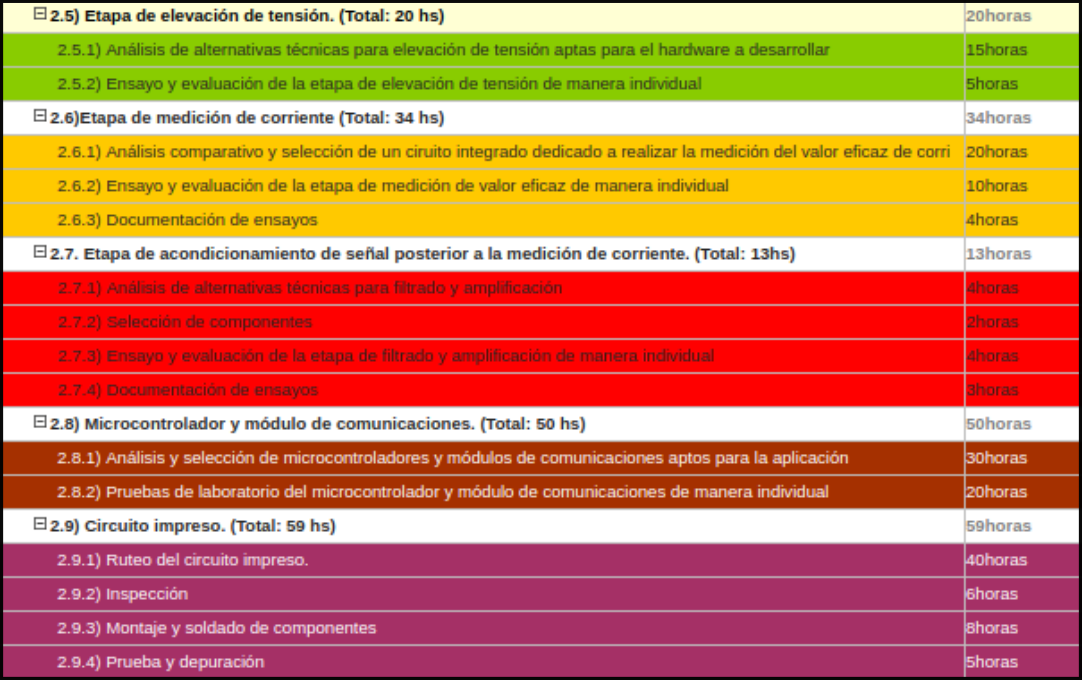
\includegraphics[width=\textwidth]{./Figuras/gantt/25-29.png}
	%\caption{Diagrama en \textit{Activity on Node}}
	\label{fig:tablegantt1}
\end{figure}
\begin{figure}[H]
	\centering 
	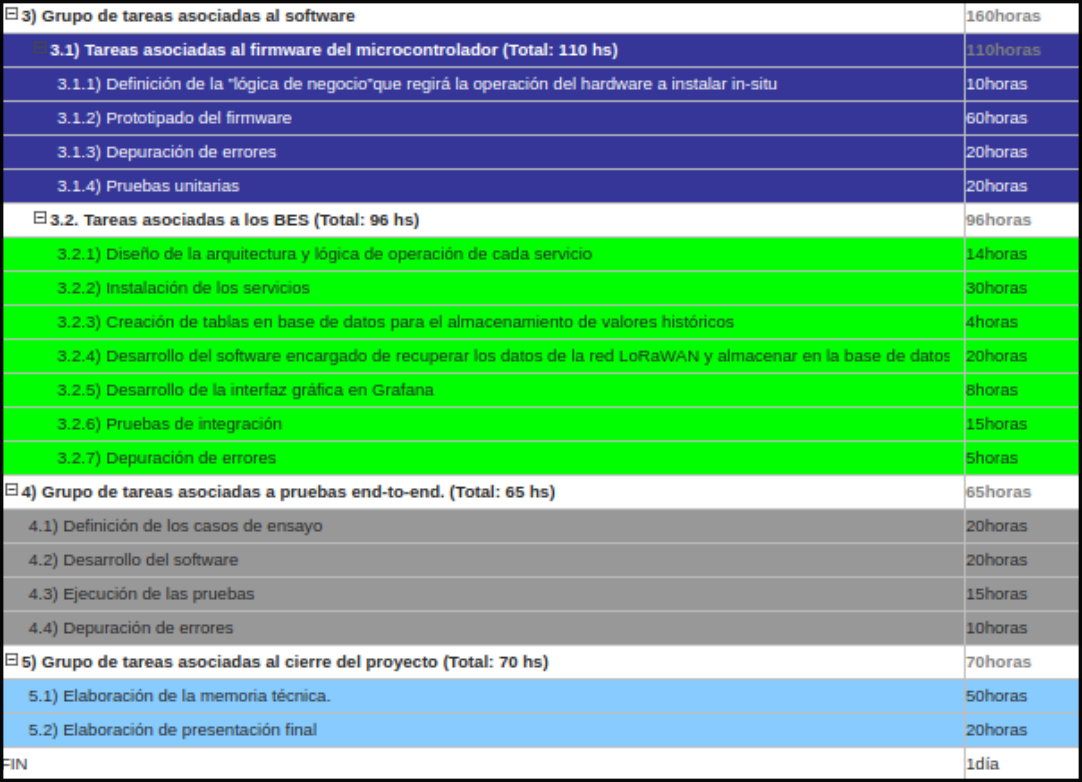
\includegraphics[width=\textwidth]{./Figuras/gantt/3-fin.png}
	\caption{Tabla para confección del diagrama de \textit{gantt}}
	\label{fig:tablegantt2}
\end{figure}
\afterpage{
\begin{landscape}
\begin{figure}[H]
	\centering 
	%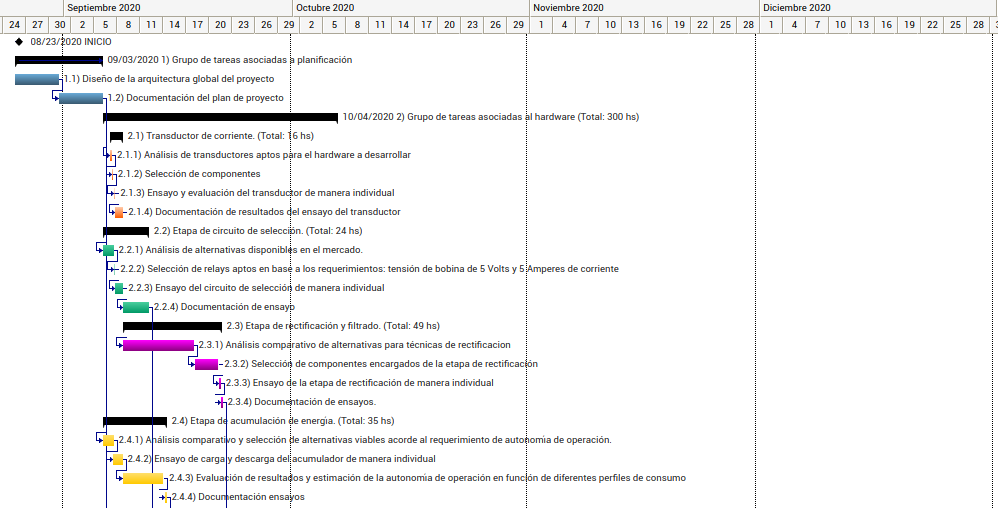
\includegraphics[width=\textwidth]{./Figuras/gantt/diagrama/gantt1-24.png}
	%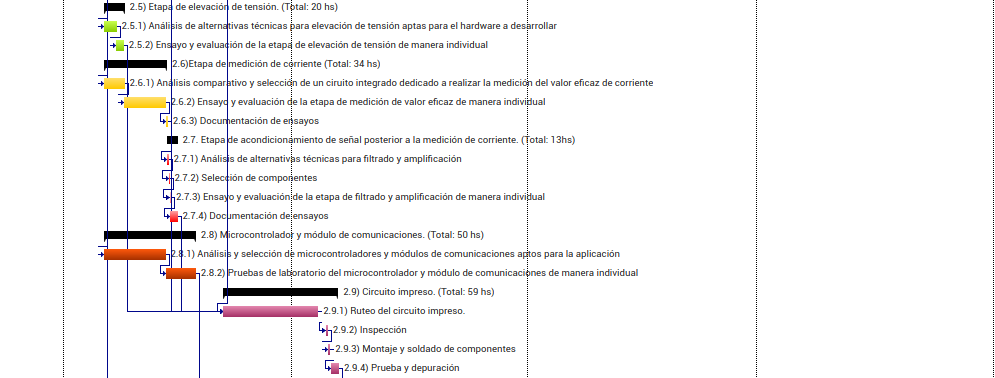
\includegraphics[width=\textwidth]{./Figuras/gantt/diagrama/gantt25-29.png}
	%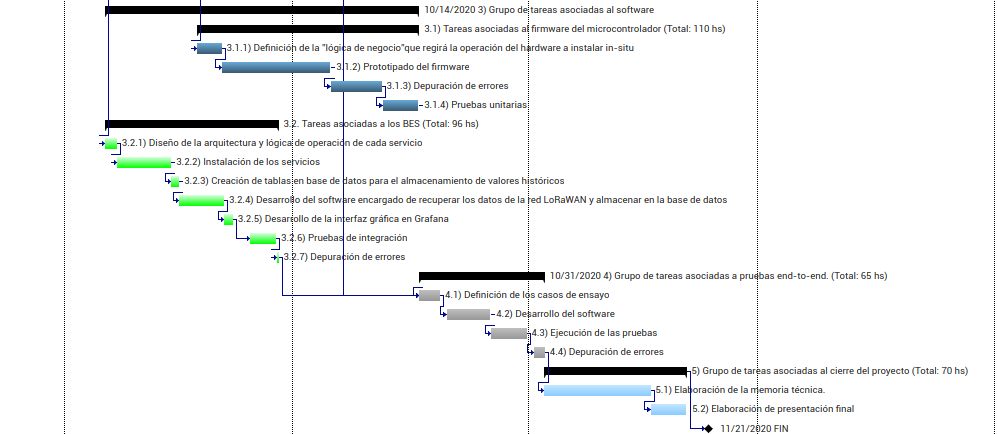
\includegraphics[width=\textwidth]{./Figuras/gantt/diagrama/gantt3-fin.png}
	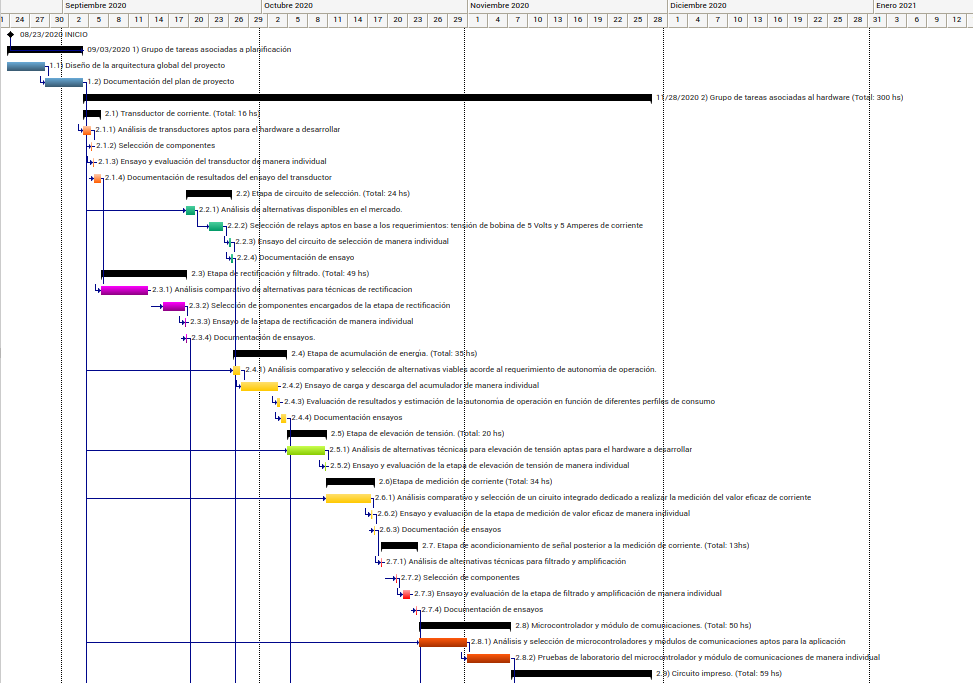
\includegraphics[width=1.35\textwidth]{./Figuras/gantt/diagrama/v2/inicio.png}
	%\includegraphics[width=\textwidth]{./Figuras/gantt/diagrama/v2/274-fin.png}
	\caption{Diagrama de \textit{gantt}}
	\label{fig:diagantt1}
\end{figure}
\begin{figure}[H]
	\centering 
	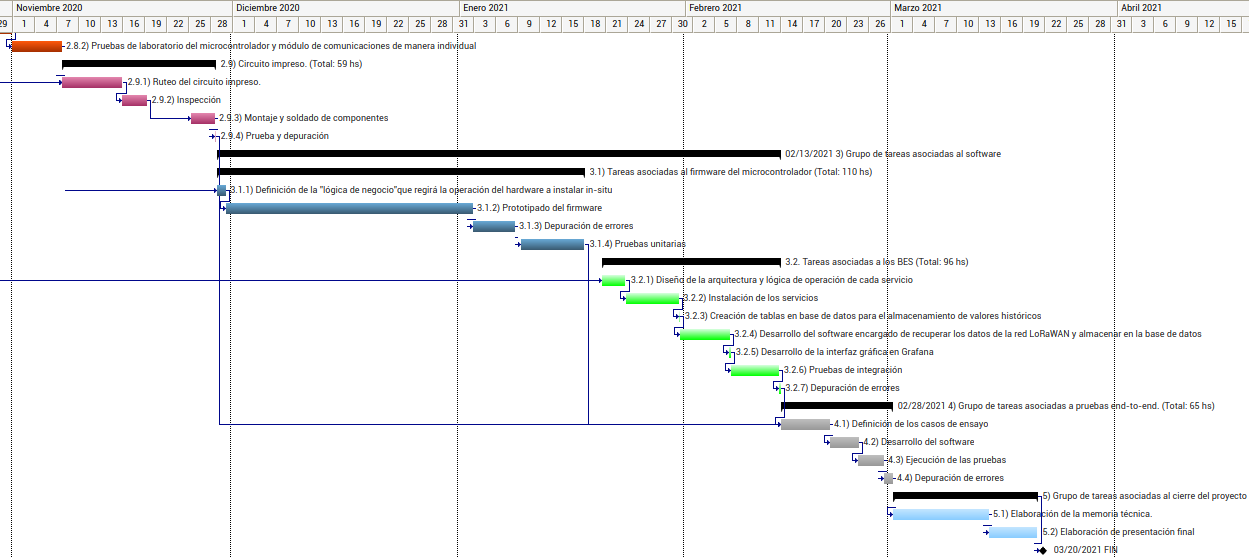
\includegraphics[width=1.5\textwidth]{./Figuras/gantt/diagrama/v2/fin.png}
	\caption{Diagrama de \textit{gantt}, continuación}
	\label{fig:diagantt2}
\end{figure}
\end{landscape}
}

\section{9. Matriz de uso de recursos de materiales}
\label{sec:recursos}

\begin{table}[H]
	\centering
	\resizebox{\textwidth}{!}{%
		\begin{tabular}{|c|c|c|c|c|c|}
			\hline
			\cellcolor[HTML]{C0C0C0} & \cellcolor[HTML]{C0C0C0} & \multicolumn{4}{c|}{\cellcolor[HTML]{C0C0C0}Recursos requeridos (horas)} \\ \cline{3-6} 
			\multirow{-2}{*}{\cellcolor[HTML]{C0C0C0}\begin{tabular}[c]{@{}c@{}}Código\\ WBS\end{tabular}} & \multirow{-2}{*}{\cellcolor[HTML]{C0C0C0}\begin{tabular}[c]{@{}c@{}}Nombre \\ tarea\end{tabular}} & PC & Laboratorio & Placa PCB & Raspberry Pi \\ \hline
	
			\rowcolor[HTML]{0000FF} 
			\textcolor{black}{1.} & \multicolumn{5}{|c|}{\textcolor{black}{Grupo de tareas asociadas a planificación}} \\ \cline{1-6}
			1.1 & Diseño de la arquitectura global & 15 &  &  &  \\ \hline
			1.2 & Documentación del plan de proyecto & 20 &  &  &  \\ \hline
	
	
			\rowcolor[HTML]{FF9E03} 
			\textcolor{black}{2.1} & \multicolumn{5}{|c|}{Transductor de corriente.} \\ \cline{1-6}
			2.1.1 & Análisis de transductores aptos para el hardware a desarrollar & 5 &  &  &  \\ \hline
			2.1.2 & Selección de componentes & 3 &  &  &  \\ \hline
			2.1.3 & Ensayo y evaluación del transductor de manera individual & 4 & 4 &  &  \\ \hline
			2.1.4 & Documentación de resultados del ensayo del transductor & 4 &  &  &  \\ \hline
	
	
			\rowcolor[HTML]{5BB576} 
			\textcolor{black}{2.2} & \multicolumn{5}{|c|}{Etapa de circuito de selección} \\ \cline{1-6}
			2.2.1 & Análisis de alternativas disponibles en el mercado & 10 &  &  &  \\ \hline
			2.2.2 & Selección de relays aptos en base a los requerimientos & 6 &  &  &  \\ \hline
			2.2.3 & Ensayo del circuito de selección de manera individual & 4 & 4 &  &  \\ \hline
			2.2.4 & Documentación de ensayo & 4 &  &  &  \\ \hline
	
	
			\rowcolor[HTML]{A232ED} 
			\textcolor{black}{2.3} & \multicolumn{5}{|c|}{Etapa de rectificación y filtrado} \\ \cline{1-6}
			2.3.1 & Análisis comparativo de alternativas para técnicas de rectificacion & 30 &  &  &  \\ \hline
			2.3.2 & Selección de componentes encargados de la etapa de rectificación & 10 &  &  &  \\ \hline
			2.3.3 & Ensayo de la etapa de rectificación de manera individual & 5 & 5 &  &  \\ \hline
			2.3.4 & Documentación de ensayos & 4 &  &  &  \\ \hline
	
			
			\rowcolor[HTML]{F7F42A} 
			\textcolor{black}{2.4} & \multicolumn{5}{|c|}{Etapa de acumulación de energía} \\ 	\cline{1-6}
			2.4.1 & Análisis y selección de alternativas viables acorde al requerimiento de autonomía de operación & 10 &  &  &  \\ \hline
			2.4.2 & Ensayo de carga y descarga del acumulador de manera individual & 10 & 10 &  &  \\ \hline
			2.4.3 & Evaluación de resultados y estimación de la autonomía de operación & 10 &  &  &  \\ \hline
			2.4.4 & Documentación ensayos & 5 &  &  &  \\ \hline		
			
			\rowcolor[HTML]{99F285} 
			\textcolor{black}{2.5} & \multicolumn{5}{|c|}{Etapa de elevación de tensión} \\ \cline{1-6}
			2.5.1 & Análisis de alternativas técnicas para elevación de tensión & 15 &  &  &  \\ \hline   
			2.5.2 & Ensayo y evaluación de la etapa de elevación de tensión & 5 & 5 &  &  \\ \hline 		
			
			
			\rowcolor[HTML]{FBFF00} 
			\textcolor{black}{2.6}& \multicolumn{5}{|c|}{Etapa de medición de corriente} \\ \cline{1-6}		
			2.6.1 & Análisis y selección de un chip dedicado a realizar la medición RMS de corriente & 20 &  &  &  \\ \hline
			2.6.2 & Ensayo de la etapa de medición de valor RMS & 10 & 10 &  &  \\ \hline   
			2.6.3 & Documentación de ensayos & 4 &  &  &  \\ \hline
		
			
			\rowcolor[HTML]{FF3650} 
			\textcolor{black}{2.7}& \multicolumn{5}{|c|}{Etapa de acondicionamiento de señal posterior a la medición de corriente} \\ \cline{1-6}		
			2.7.1 & Análisis de alternativas técnicas para filtrado y amplificación & 4 &  &  &  \\ \hline
			2.7.2 & Selección de componentes & 2 &  &  &  \\ \hline   
			2.7.3 & Ensayo de la etapa de filtrado y amplificación & 4 & 4 &  &  \\ \hline   
			2.7.4 & Documentación de ensayos & 3 &  &  &  \\ \hline
	
			
			\rowcolor[HTML]{D48B1E} 
			\textcolor{black}{2.8}& \multicolumn{5}{|c|}{Microcontrolador y módulo de comunicaciones} \\ \cline{1-6}		
			2.8.1 & Análisis y selección de microcontroladores y módulos de comunicaciónes & 30 &  &  &  \\ \hline   
			2.8.2 & Pruebas de laboratorio del microcontrolador y módulo de comunicaciónes & 20 & 20 &  &  \\ \hline
	
			
			\rowcolor[HTML]{B34791} 
			\textcolor{black}{2.9}& \multicolumn{5}{|c|}{Circuito impreso} \\ \cline{1-6}		   
			2.9.1 & Ruteo del circuito impreso & 40 &  &  &  \\ \hline   
			2.9.2 & Inspección & 6 &  &  &  \\ \hline    
			2.9.3 & Montaje y soldado de componentes & 8 & 8 & 8 &  \\ \hline
			2.9.4 & Prueba y depuración & 5 & 5 & 5 &  \\ \hline		
	
			
			\rowcolor[HTML]{0A12FC} 
			\textcolor{black}{3.1} & \multicolumn{5}{|c|}{Tareas asociadas al firmware del microcontrolador} \\ \cline{1-6}		   
			3.1.1 & Definición de la ”lógica de negocio”que regirá la operación del hardware & 10 &  &  &  \\ \hline   
			3.1.2  & Prototipado del firmware & 60 &  &  &  \\ \hline   
			3.1.3  & Depuración de errores & 20 &  &  &  \\ \hline
			3.1.4  & Pruebas unitarias & 20 &  &  &  \\ \hline
	
		
			\rowcolor[HTML]{95FF00} 
			\textcolor{black}{3.2} & \multicolumn{5}{|c|}{Tareas asociadas los BES} \\ \cline{1-6}		   
			3.2.1  & Diseño de la arquitectura y lógica de operación de cada servicio & 14 &  &  &  \\ \hline   
			3.2.2  & Instalación de los servicios & 30 &  &  & 30 \\ \hline   
			3.2.3  & Creación de tablas en base de datos para el almacenamiento de valores históricos & 4 &  &  & 4 \\ \hline   
			3.2.4  & Desarrollo del software encargado de recuperar los datos de la red LoRaWAN & 20 &  &  & 20 \\ \hline
			3.2.5  & Desarrollo de la interfaz gráfica en Grafana & 8 &  &  & 8 \\ \hline   
			3.2.6  & Pruebas de integración & 15 &  &  & 15 \\ \hline
			3.2.7  & Depuración de errores & 5 &  &  & 5 \\ \hline
			
			
			\rowcolor[HTML]{B8BAB5} 
			\textcolor{black}{4} & \multicolumn{5}{|c|}{Grupo de tareas asociadas a pruebas end-to-end} \\ \cline{1-6}		   
			4.1  & Definición de los casos de ensayo & 20 &  &  &  \\ \hline   
			4.2  & Desarrollo del software & 20 &  &  & 20 \\ \hline
			4.3  & Ejecución de las pruebas & 15 & 15 & 15 & 15 \\ \hline   
			4.4  & Depuración de errores & 10 & 10 & 10 & 10 \\ \hline
			
			
			\rowcolor[HTML]{ADF3FF} 
			\textcolor{black}{5} & \multicolumn{5}{|c|}{Grupo de tareas asociadas al cierre del proyecto} \\ \cline{1-6}		   
			5.1  & Elaboración de la memoria técnica & 50 &  &  &  \\ \hline   
			5.2  & Elaboración de la presentación final & 20 &  &  &  \\ \hline
	
	
			\rowcolor[HTML]{C0C0C0} 
			\multicolumn{2}{|c|}{\cellcolor[HTML]{C0C0C0} Totales} &676 hs & 100 hs &38  hs &  127 hs \\ \hline
		\end{tabular}%
	}
\end{table}

{\footnotesize
	Referencias:
	\begin{itemize}
		\item PC = Computadora personal con todo el software necesario para el desarrollo de proyecto.
		\item Laboratorio = Espacio físico donde se realizaran diferentes ensayos.
		\item Placa PCB = Circuito impreso del prototipo a desarrollar.
		\item Raspberry Pi = Computadora de bajo costo donde correran los BES.
	\end{itemize}
} %footnotesize

\section{10. Presupuesto detallado del proyecto}
\label{sec:presupuesto}
Los precios expresados en la siguiente tabla se encuentran en Euros \euro{}.\\

\begin{table}[htpb]
\centering
\begin{tabularx}{\linewidth}{@{}|X|c|r|r|@{}}
\hline
\rowcolor[HTML]{C0C0C0} 
\multicolumn{4}{|c|}{\cellcolor[HTML]{C0C0C0}COSTOS DIRECTOS} \\ \hline
\rowcolor[HTML]{C0C0C0} 
Descripción &
  \multicolumn{1}{c|}{\cellcolor[HTML]{C0C0C0}Cantidad} &
  \multicolumn{1}{c|}{\cellcolor[HTML]{C0C0C0}Valor unitario} &
  \multicolumn{1}{c|}{\cellcolor[HTML]{C0C0C0}Valor total} \\ \hline

 Transformador de intensidad tipo núcleo partido y clase 0.5&
  \multicolumn{1}{c|}{1} &
  \multicolumn{1}{c|}{92.00} &
  \multicolumn{1}{c|}{92.00} \\ \hline

 Circuito impreso &
 \multicolumn{1}{c|}{1} &
 \multicolumn{1}{c|}{40.00} &
 \multicolumn{1}{c|}{40.00} \\ \hline

 Componentes electrónicos varios * &
 \multicolumn{1}{c|}{1} &
 \multicolumn{1}{c|}{100.00} &
 \multicolumn{1}{c|}{100.00} \\ \hline

 Módulo de desarrollo basado en ESP32 y transceptor LoRa *&
 \multicolumn{1}{c|}{1} &
 \multicolumn{1}{c|}{40.00} &
 \multicolumn{1}{c|}{40.00} \\ \hline

 Raspberry Pi 3 B+&
  \multicolumn{1}{c|}{1} &
  \multicolumn{1}{c|}{45.00} &
  \multicolumn{1}{c|}{45.00} \\ \hline
  
 Acumulador&
 \multicolumn{1}{c|}{1} &
 \multicolumn{1}{c|}{10.00} &
 \multicolumn{1}{c|}{10.00} \\ \hline 

 Viáticos de movilidad&
 \multicolumn{1}{c|}{1} &
 \multicolumn{1}{c|}{600.00} &
 \multicolumn{1}{c|}{600.00} \\ \hline 
 

 Honorarios profesionales&
 \multicolumn{1}{c|}{676} &
 \multicolumn{1}{c|}{10} &
 \multicolumn{1}{c|}{6760.00} \\ \hline


\multicolumn{3}{|c|}{SUBTOTAL} &
  \multicolumn{1}{c|}{7687.00} \\ \hline
\rowcolor[HTML]{C0C0C0} 
\multicolumn{4}{|c|}{\cellcolor[HTML]{C0C0C0}COSTOS INDIRECTOS} \\ \hline
\rowcolor[HTML]{C0C0C0} 
Descripción &
  \multicolumn{1}{c|}{\cellcolor[HTML]{C0C0C0}Cantidad} &
  \multicolumn{1}{c|}{\cellcolor[HTML]{C0C0C0}Valor unitario} &
  \multicolumn{1}{c|}{\cellcolor[HTML]{C0C0C0}Valor total} \\ \hline

\multicolumn{1}{|l|}{Multímetro digital True RMS}
	&
   1&
   100.00&
   100.00\\ \hline
   
   
\multicolumn{1}{|l|}{Generador de señales} &
1&
80.00&
80.00\\ \hline


\multicolumn{1}{|l|}{Servicios de energía eléctrica e internet} &
1&
70.00&
70.00\\ \hline
   
\multicolumn{3}{|c|}{SUBTOTAL} &
  \multicolumn{1}{c|}{250.00} \\ \hline
\rowcolor[HTML]{C0C0C0}
\multicolumn{3}{|c|}{TOTAL} &
   7937.00\\ \hline
\end{tabularx}%
\end{table}
\euro{7937} = 887.356 Pesos Argentinos*\\
(*) Valores aproximados

\section{11. Matriz de asignación de responsabilidades}
\label{sec:responsabilidades}

\begin{table}[H]
\centering
\resizebox{\textwidth}{!}{%
\begin{tabular}{|c|c|c|c|c|c|}
\hline
\rowcolor[HTML]{C0C0C0} 
\cellcolor[HTML]{C0C0C0} &
  \cellcolor[HTML]{C0C0C0} &
  \multicolumn{4}{c|}{\cellcolor[HTML]{C0C0C0}Listar todos los nombres y roles del proyecto} \\ \cline{3-6} 
\rowcolor[HTML]{C0C0C0} 
\cellcolor[HTML]{C0C0C0} &
  \cellcolor[HTML]{C0C0C0} &
  Responsable &
  Orientador &
  Colaborador &
  Cliente \\ \cline{3-6} 
\rowcolor[HTML]{C0C0C0} 
\multirow{-3}{*}{\cellcolor[HTML]{C0C0C0}\begin{tabular}[c]{@{}c@{}}Código\\ WBS\end{tabular}} &
  \multirow{-3}{*}{\cellcolor[HTML]{C0C0C0}Nombre de la tarea} &
  \authorname &
  \supname &
  Ing. Germán A. Xánder &
  \clientename \\ \hline
   1.1& Diseño de la arquitectura global  & P & A & C & A \\ \hline
   1.2& Documentación del plan de proyecto & P & A/C & C & A \\ \hline
 2.1.1& Análisis de transductores aptos para el hardware a desarrollar & P & C/A & C &  \\ \hline
 2.1.2& Selección de componentes & P & C & C & I \\ \hline
 2.1.3& Ensayo y evaluación del transductor de manera individual & P & C/A & C &  \\ \hline
 2.1.4& Documentación de resultados del ensayo del transductor & P & A &  &  \\ \hline
 2.2.1& Análisis de alternativas disponibles en el mercado & P &  &  &  \\ \hline
 2.2.2& Selección de relays aptos en base a los requerimientos & P & C/A & C &  \\ \hline
 2.2.3& Ensayo del circuito de selección de manera individual & P &  &  &  \\ \hline
 2.2.4& Documentación de ensayo & P & A &  &  \\ \hline
 2.3.1& Análisis comparativo de alternativas para técnicas de rectificacion & P & C & C &  \\ \hline
 2.3.2& Selección de componentes encargados de la etapa de rectificación & P & C/A & C &  \\ \hline
 2.3.3& Ensayo de la etapa de rectificación de manera individual & P &  &  &  \\ \hline
 2.3.4& Documentación de ensayos & P & A &  &  \\ \hline
 2.4.1& Análisis y selección de alternativas viables acorde al requerimiento de autonomía de operación & P & C &  &  \\ \hline
 2.4.2& Ensayo de carga y descarga del acumulador de manera individual & P &  &  &  \\ \hline
 2.4.3& Evaluación de resultados y estimación de la autonomía de operación & P & C &  &  \\ \hline
 2.4.4& Documentación ensayos & P & A &  &  \\ \hline
 2.5.1& Análisis de alternativas técnicas para elevación de tensión & P &  &  &  \\ \hline
 2.5.2& Ensayo y evaluación de la etapa de elevación de tensión & P & C &  &  \\ \hline
 2.6.1& Análisis y selección de un chip dedicado a realizar la medición RMS de corriente & P & C & C &  \\ \hline
 2.6.2& Ensayo de la etapa de medición de valor RMS & P &  &  &  \\ \hline
 2.6.3& Documentación de ensayos & P & A &  &  \\ \hline
 2.7.1& Análisis de alternativas técnicas para filtrado y amplificación & P & C & C &  \\ \hline
 2.7.2& Selección de componentes & P & C/A & C &  \\ \hline
 2.7.3& Ensayo de la etapa de filtrado y amplificación & P &  &  &  \\ \hline
 2.7.4& Documentación de ensayos & P & A &  &  \\ \hline
 2.8.1& Análisis y selección de microcontroladores y módulos de comunicaciónes & P &  &  &  \\ \hline
 2.8.2& Pruebas de laboratorio del microcontrolador y módulo de comunicaciónes & P &  &  &  \\ \hline
 2.9.1& Ruteo del circuito impreso & P & A &  &  \\ \hline
 2.9.2& Inspección & P & C & C &  \\ \hline
 2.9.3& Montaje y soldado de componentes & P &  &  &  \\ \hline
 2.9.4& Prueba y depuración & P &  &  &  \\ \hline
 3.1.1& Definición de la ”lógica de negocio”que regirá la operación del hardware & P & C &  & A \\ \hline
 3.1.2& Prototipado del firmware & P & C &  &  \\ \hline
 3.1.3& Depuración de errores & P &  &  &  \\ \hline
 3.1.4& Pruebas unitarias & P &  &  &  \\ \hline
 3.2.1& Diseño de la arquitectura y lógica de operación de cada servicio & P & C & C & A \\ \hline
 3.2.2& Instalación de los servicios & P &  & C &  \\ \hline
 3.2.3& Creación de tablas en base de datos para el almacenamiento de valores históricos & P &  & C &  \\ \hline
 3.2.4& Desarrollo del software encargado de recuperar los datos de la red LoRaWAN & P &  & C &  \\ \hline
 3.2.5& Desarrollo de la interfaz gráfica en Grafana & P & C/A &  & A \\ \hline
 3.2.6& Pruebas de integración & P &  &  &  \\ \hline
 3.2.7& Depuración de errores & P &  &  &  \\ \hline
 4.1& Definición de los casos de ensayo & P & C/A &  & A \\ \hline
 4.2& Desarrollo del software & P & C & C &  \\ \hline
 4.3& Ejecución de las pruebas & P &  &  &  \\ \hline
 4.4& Depuración de errores & P & C &  &  \\ \hline
 5.1& Elaboración de la memoria técnica & P & A & C &  \\ \hline
 5.2& Elaboración de la presentación final & P & A & I & I \\ \hline
\end{tabular}%
}
\end{table}
{\footnotesize
Referencias:
\begin{itemize}
	\item P = Responsabilidad Primaria
	\item A = Aprobación
	\item I = Informado
	\item C = Consultado
\end{itemize}
} %footnotesize


\section{12. Gestión de riesgos}
\label{sec:riesgos}

\begin{consigna}{black}
a) Identificación de los riesgos (al menos cinco) y estimación de sus consecuencias:
 
Riesgo 1: Falta de tiempo para terminar con todas las tareas estipuladas en el desglose de trabajo en tareas.
\begin{itemize}
\item Severidad (6): se demoraría la entrega de toda la documentación y la presentación final.\\
\item Probabilidad de ocurrencia (3): un desglose detallado de tareas permite programar una reasignación de prioridades mientras se mitigan los impactos.\\
\end{itemize}   

Riesgo 2: No poder conseguir los materiales.
\begin{itemize}
\item Severidad (5): De no conseguir circuitos integrados especificos, se deberá realizar una alternativa de tipo casera con componentes discretos que cumpla con las mismas especificaciones.
\item Probabilidad de ocurrencia (2): los componentes asociados a la etapa de hardware no son dificiles de conseguir, sin embargo, un proceso lento de exportación de los mismos es dable.
\end{itemize}


Riesgo 3: Falla en el circuito impreso
\begin{itemize}
\item Severidad (5): demoraría el comienzo de las pruebas end-to-end.
\item Probabilidad de ocurrencia (3): se deberá ensayar previamente todo en un protoboard. Si funcionase sin problemas en el protoboard, la posibilidad de fallo se reduce.
\end{itemize}


Riesgo 4: Los servicios de backend privados especificos del proyecto se encuentran caídos al momento de realizar ensayos end-to-end.
\begin{itemize}
	\item Severidad (4): de no estar operativos los BES, no se podrá probar la GUI en grafana. Sin embargo, se podra verificar que los datos lleguen a la red LoRaWAN.
	\item Probabilidad de ocurrencia (2): los servicios de BES son unicamente 3 y poseen mecanismos de monitoreo de estado antes de comenzar con los ensayos.
\end{itemize}


Riesgo 5: Restricciones de movilidad debido al COVID-19.
\begin{itemize}
	\item Severidad (6): no poder trasladarse hacia el laboratorio representaria un gran impacto al momento de ensayar las etapas de manera individual. También impactaría sobre la presentación final que debera hacerse de manera remota y no presencial.
	\item Probabilidad de ocurrencia (7): Los indices de casos positivos son muy dispares entre las diferentes regiones de Argentina, por lo que podrían resurgir otros brotes.
\end{itemize}

b) Tabla de gestión de riesgos:      (El RPN se calcula como RPN=SxO)

\begin{table}[htpb]
\centering
\begin{tabularx}{\linewidth}{@{}|X|c|c|c|c|c|c|@{}}
\hline
\rowcolor[HTML]{C0C0C0} 
Riesgo & S & O & RPN & S* & O* & RPN* \\ \hline
 Riesgo 1& 6 & 3 & 18  &    &    &      \\ \hline
 Riesgo 2& 5 & 2 & 10  &    &    &      \\ \hline
 Riesgo 3& 5 & 3 & 15  &    &    &      \\ \hline
 Riesgo 4& 4 & 2 & 8   &    &    &      \\ \hline
 Riesgo 5& 6 & 7 & 42  &  3  &  1  &      \\ \hline
\end{tabularx}%
\end{table}

Criterio adoptado: 
Se tomarán medidas de mitigación en los riesgos cuyos números de RPN sean mayores a 20.

Nota: los valores marcados con (*) en la tabla corresponden luego de haber aplicado la mitigación.

c) Plan de mitigación de los riesgos que originalmente excedían el RPN máximo establecido:
 
Riesgo 5: se deberá planear el armado de un laboratorio que sea portatil y posea todas las herramientas necesarias para desarrollar las pruebas. Tambien se deberá modificar la forma y contenido de la presentación del trabajo final ante el cliente y jurado por otra que integre herramientas para video conferencia.
\begin{itemize}
	\item Severidad (3): al disponer del laboratorio portatil deja de ser necesario trasladarse. También impactaría sobre la presentación final que debera hacerse de manera remota y no presencial.
	\item Ocurrencia (1): Se espera que los brotes de Los indices de casos positivos son muy dispares entre las diferentes regiones de Argentina, por lo que podrían resurgir otros brotes.
\end{itemize}

\end{consigna}

\section{13. Gestión de la calidad}
\label{sec:calidad}

\begin{consigna}{black}
Para cada uno de los requerimientos del proyecto indique:
%\begin{itemize} 
%\item Req: Copiar acá el requerimiento.
\begin{enumerate}
	\item Grupo de requerimientos asociados con hardware
	\begin{enumerate}[label*=\arabic*.]
			\item El dispositivo deberá ser de tipo \textit{plug and play}.
				\begin{itemize}
					\item Verificación: una vez finalizado el hardware, la unica acción necesaria será instalar el transformador de corriente sobre el conductor.\\
					\item Validación: el cliente en persona hará una prueba de comisionamiento y puesta en funcionamiento.\\
				\end{itemize}
				
			\item El circuito impreso no deberá ocupar un volumen mayor a 10x10x5 cm.
				\begin{itemize}
					\item Verificación: se verificará el diseño de la placa antes de mandar al fabricante.\\
					\item Validación: el cliente tendrá siempre acceso al esquematico, los diseños y hojas de datos de los componentes.\\
				\end{itemize}
				
			\item Basarse en un microcontrolador ESP32 y disponer de:
			\begin{enumerate}[label*=\arabic*.]
				\item 4 entradas analógicas.
					\begin{itemize}
							\item Verificación: entre las variantes disponibles se seleccionará aquella que cumpla con este requisito.\\
							\item Validación: se harán pruebas de laboratorio utilizando un potenciómetro.\\
					\end{itemize}
				\item 3 salidas digitales.
					\begin{itemize}
						\item Verificación: entre las variantes disponibles se seleccionará aquella que cumpla con este requisito.\\
						\item Validación: se harán pruebas de laboratorio usando leds y pulsadores.\\
					\end{itemize}
				\item Unidad UART.
					\begin{itemize}
						\item Verificación: entre las variantes disponibles se seleccionará aquella que cumpla con este requisito.\\
						\item Validación: se harán pruebas de laboratorio usando un adaptador UART-USB.\\
					\end{itemize}
				\item Integrar un módulo de comunicaciones LoRa.
					\begin{itemize}
						\item Verificación: en caso de no encontrarse un modulo del microcontrolador que ya lo integre, se usará un módulo a parte.\\
						\item Validación: se harán pruebas de laboratorio contra la red LoRaWAN.\\
					\end{itemize}
			\end{enumerate}
			
			\item Deberá tener al menos 12 horas de autonomía de funcionamiento.
				\begin{itemize}
					\item Verificación: se realizará una prueba de laboratorio para exponer su máxima autonomia.\\
					\item Validación: se planificará un ensayo junto con el cliente de manera presencial.\\
				\end{itemize}
			
			\item Bajo consumo en modo ocioso: el consumo del hardware en total, no deberá superar los 5 mA cuando no está midiendo ni transmitiendo.
				\begin{itemize}
					\item Verificación: se verificarán que todas las etapas del hardware esten en modo ahorro de energía o desactivadas.\\
					\item Validación: se realizará una medición de corriente a la salida del acumulador.\\
				\end{itemize}
				
			\item El circuito elevador de tensión DC-DC deberá:
			\begin{enumerate}[label*=\arabic*.]
				\item Funcionar con tensiones menores a 2V en la entrada.
					\begin{itemize}
						\item Verificación: se buscarán módulos cuyas hojas de datos cumplan con este requisito.\\
						\item Validación: mediante una fuente regulable se verificará que el circuito elevador comience a funcionar con menos de 2.\\
					\end{itemize}
					
				\item Otorgar 5 Volts a la salida.
					\begin{itemize}
						\item Verificación: se buscará en su hoja de datos la tensión de salida nominal.\\
						\item Validación: se energizará al circuito elevador mediante una fuente regulable y se conectará a la salida un multímetro para medir este valor.\\
					\end{itemize}
					
				\item Ser capaz de otorgar 300 miliamperes a la salida.
					\begin{itemize}
						\item Verificación: se buscará en su hoja de datos su corriente máxima de salida.\\
						\item Validación: se energizará al circuito elevador mediante una fuente regulable y se conectará a la salida una carga resistiva de 16 Ohms y medirá su corriente.\\
					\end{itemize}
			\end{enumerate}
			
			\item El transformador de corriente debe:
			\begin{enumerate}[label*=\arabic*.]
				\item Ser de tipo núcleo partido.
					\begin{itemize}
						\item Verificación: al momento de seleccionarlo se analizaran las variantes con o sin bisagras.\\
						\item Validación: el cliente recibirá la hoja de datos del transformador de corriente seleccionado.\\
					\end{itemize}
				\item Admitir 100 Amperes de corriente en el circuito primario y un máximo 5 Amperes en el circuito secundario.
					\begin{itemize}
						\item Verificación: al momento de seleccionarlo se analizará la hoja de datos de las posibles variantes que cumplan con los requisitos.\\
						\item Validación: el cliente recibirá la hoja de datos del transformador de corriente seleccionado.\\
					\end{itemize}
			\end{enumerate}
			
			\item El relay encargado de cambiar el modo de operación debe:
			\begin{enumerate}[label*=\arabic*.]
				\item Ser de tipo doble invesor sin retención.
					\begin{itemize}
						\item Verificación: se utilizarán las hojas de datos de los fabricantes.\\
						\item Validación: se realizará un ensayo de laboratorio con dos leds y un pulsador.\\
					\end{itemize}
				\item Su bobina debe poder energizarse con 5V o menos.
					\begin{itemize}
						\item Verificación: se consultarán las hojas de datos del fabricante.\\
						\item Validación: se realizará un ensayo de laboratorio con una fuente regulable incrementando su valor de manera progresiva.\\
					\end{itemize}
				\item Soportar al menos 5 Amperes de corriente por los contactos.
					\begin{itemize}
						\item Verificación: se consultarán las hojas de datos del fabricante.\\
						\item Validación: se realizará un ensayo de laboratorio con una carga fantasma.\\
					\end{itemize}
			\end{enumerate}
			
			\item Debe funcionar de manera independiente a la frecuencia de operación de la red 50/60 Hz.
				\begin{itemize}
					\item Verificación: al seleccionar el transductor y el chip medidor de corriente se verificará que ambos cumplan con este requerimiento.\\
					\item Validación: el cliente proveerá un variador de frecuencia al momento de hacer ensayos sobre 60 Hz.\\
				\end{itemize}
			
			\item Debe funcionar de manera independiente a la tensión de fase del sistema de distribución 110/220 Voltios.
				\begin{itemize}
					\item Verificación: al seleccionar el transductor y el chip medidor de corriente se verificará que ambos cumplan con este requerimiento.\\
					\item Validación: se haran pruebas conectando cargas a una tensíon de 110 Volts provista por un transformador de potencia.\\
				\end{itemize}			

	\end{enumerate}
	\item Grupo de requerimientos asociados con el firmware
		\begin{enumerate}[label*=\arabic*.]
			\item Debe manejar un módulo de comunicación LoRa y protocolo LoRaWAN.
				\begin{itemize}
					\item Verificación: se buscarán bibliotecas aptas para el manejo del protocolo.\\
					\item Validación: se hará una prueba de laboratorio enviando datos a la red LoRaWAN.\\
				\end{itemize}
			\item Deberá tener un porcentaje de cobertura de tests unitarios del 60 por ciento como mínimo.
				\begin{itemize}
					\item Verificación: se analizaran cuantas funciona se desarrollaron y cuantas pruebas unitarias.\\
					\item Validación: El cliente podrá acceder a un reporte de cobertura como así también al código.\\
				\end{itemize}
			\item Antes configurarse en modo ocioso, debe desenergizar la etapa de medición de corriente y el módulo de comunicaciones con el objeto de ahorrar energía.
				\begin{itemize}
					\item Verificación: se consultara en hojas de datos de cada etapa los consumos en cada modo.\\
					\item Validación: se medirá el consumo total del circuito al entrar en ahorro de energia.\\
				\end{itemize}
		\end{enumerate}
	\item Grupo de requerimientos asociados con los BES
		\begin{enumerate}[label*=\arabic*.]
			\item Todos los servicios deben poder correr en una Raspberry Pi 3.
			\begin{itemize}
				\item Verificación: Antes de comenzar con la instalación se verificará que los servicios pueden correr sobre la arquitectura del dispositivo.\\
				\item Validación: junto al cliente se realizarán pruebas de comunicación entre los BES.\\
			\end{itemize}
			
			\item El software de los BES se desarrollará en lenguaje Python.
			\begin{itemize}
				\item Verificación: se solicitará asesoría al tutor y colaboradores para el desarrollo necesario.\\
				\item Validación: sin acción asociada.\\
			\end{itemize}
			
			\item Recuperar los datos de la red LoRaWAN.
			\begin{itemize}
				\item Verificación: Se hará uso de los logs de la API de recuperación de datos.\\
				\item Validación: el cliente enviará datos desde un hardware de prueba a la red LoRaWAN y con el objeto de validar el mecanismo de recuperación se observarán los logs en los BES.\\
			\end{itemize}

			\item Almacenar los datos en una tabla de MySQL.
			\begin{itemize}
				\item Verificación: se implementarán tablas para el almacenamiento de los datos historicos y vistas para obtener los ultimos datos.\\
				\item Validación: el cliente enviará datos desde un hardware de prueba a la red LoRaWAN y verificará que los mismos se almacenen en la base de datos accediendo a las tablas.\\
			\end{itemize}
			
			\item GUI basada en Grafana.
			\begin{itemize}
				\item Verificación: Se verificará una vez elaborado el dashboard, que se muestren los ultimos datos recolectados de cada nodo en la base de datos.\\
				\item Validación: el cliente enviará datos desde un hardware de prueba la red LoRaWAN y simultaneamente tendrá acceso a la GUI.\\
			\end{itemize}
		\end{enumerate}
		
	\item Grupo de requerimientos asociados con ensayos de integración y end-to-end.
		\begin{enumerate}[label*=\arabic*.]
			\item El banco de ensayos de hardware debe contar con una carga fantasma de al menos
			10 Amperes y permitir realizar interrupciones de corriente de manera programada
			mediante una computadora adicional tipo Raspberry Pi o de manera manual.
			\begin{itemize}
				\item Verificación: el banco de prueba constara de una estufa halogena de al menos 2200 Watts y será accionada mediante un relay o contactor.\\
				\item Validación: el cliente podrá probar el banco de ensayos y validar las mediciones con una pinza amperométrica el mismo.\\
			\end{itemize}
			
			\item Los BES deben estar operativos al momento de realizar los ensayos.
			\begin{itemize}
				\item Verificación: se haran monitoreo de estado y alertas de manera automatica.\\
				\item Validación: el cliente podrá acceder a todos los servicios de backend de manera remota en todo momento.\\
			\end{itemize}
			
			\item Contar con un gateway de acceso a una red LoRaWAN como por ejemplo \textit{The Things Network}.
			\begin{itemize}
				\item Verificación: se contara con un gateway multicanal TTIG-915.\\
				\item Validación: el cliente tendrá a dispoción dicho equipo en todo momento.\\
			\end{itemize}
		\end{enumerate}
\end{enumerate}

\end{consigna}

\section{14. Comunicación del proyecto}
\label{sec:comunicaciones}

\begin{consigna}{black}
El plan de comunicación del proyecto es el siguiente:
\end{consigna}

% Please add the following required packages to your document preamble:
% \usepackage{graphicx}
% \usepackage[table,xcdraw]{xcolor}
% If you use beamer only pass "xcolor=table" option, i.e. \documentclass[xcolor=table]{beamer}
\begin{table}[htpb]
\centering
\resizebox{\textwidth}{!}{%
\begin{tabular}{|c|c|c|c|c|c|}
\hline
\rowcolor[HTML]{C0C0C0} 
\multicolumn{6}{|c|}{\cellcolor[HTML]{C0C0C0}PLAN DE COMUNICACIÓN DEL PROYECTO}           \\ \hline
\rowcolor[HTML]{C0C0C0} 
¿Qué comunicar? &Audiencia & Propósito&Frecuencia& Método de comunicac. & Responsable \\ \hline
     Alcance del proyecto &Director&Definir los limites del proyecto&Al inciar el proyecto&Video-conferencia&Milton Sosa\\ \hline
     Avances &Director&Cada dos semanas& Comunicar avances & Video-conferencia & Milton Sosa  \\ \hline
     Consultas Técnicas& Director y Colaboradores&Acalarar dudas técnicas&Bajo demanda& Video-conferencia o mailo &Milton Sosa\\ \hline
     Cierre del proyecto&Cliente y Jurado&Evualuar y finalizar el proyecto&Una vez al finalizar el proyecto&Presentación online o presencial&Milton Sosa\\ \hline
\end{tabular}%
}
\end{table}

\section{15. Gestión de Compras}
\label{sec:compras}

\begin{consigna}{black}
Al realizar compras de insumos de cualquier tipo, se priorizarán a proveedores que aseguren un tiempo de entrega menor a 10 días.
\begin{itemize}
\item Proveedor: Digi-Key, Reichelt GmbH o Amazon.
\item Criterio de elección: variedad y disponibilidad de componentes, ventas a nivel minorista, rápida entrega a Alemania y gestiones de aduana ya incluídas.
\end{itemize}
\end{consigna}

\section{16. Seguimiento y control}
\label{sec:seguimiento}
\begin{table}[H]
\centering
\begin{tabularx}{\linewidth}{@{}|X|X|X|X|X|X|@{}}
\hline
\rowcolor[HTML]{C0C0C0} 
\multicolumn{6}{|c|}{\cellcolor[HTML]{C0C0C0}SEGUIMIENTO DE AVANCE}                                                                       \\ \hline
\rowcolor[HTML]{C0C0C0} 
Tarea del WBS & Indicador de avance & Frecuencia de reporte & Resp. de seguimiento & Persona a ser informada & Método de comunic. \\ \hline
 1&Entregas semanales& Semanal&Milton Sosa& Director y docente del CESE&Mail\\ \hline
 2.1&Qué transductor se ha elegido y ensayado&Quincenal&Milton Sosa&Director&Video-conferencia, mail\\ \hline
 2.2&Cuántos relays aptos se encontraron y ensayaron.&Quincenal&Milton Sosa&Director&Video-conferencia, mail\\ \hline
 2.3&Qué técnica de rectificación se ha adoptado y que componentes se utilizará&Quincenal&Milton Sosa&Director& Video-conferencia, mail\\ \hline
 2.4&Qué alternativa se adoptó y cual es la autonomía estimada&Quincenal&Milton Sosa&Director&Video-conferencia, mail\\ \hline
 2.5&Qué alternativa se ha adoptado&Quincenal&Milton Sosa&Director&Video-conferencia, mail\\ \hline
 2.6&Qué chip se ha adoptado&Quincenal&Milton Sosa&Director&Video-conferencia, mail\\ \hline
 2.7&Qué circuito se adoptará y que componentes se utilizarán&Quincenal&Milton Sosa&Director&Video-conferencia, mail\\ \hline
 2.8&Que placa de desarrollo y módulo de comunicaciones se utilizará&Quincenal&Milton Sosa&Director&Video-conferencia, mail\\ \hline
\end{tabularx}%
%}
\end{table}


\begin{table}[H]
	\centering
	\begin{tabularx}{\linewidth}{@{}|X|X|X|X|X|X|@{}}
		\hline
		\rowcolor[HTML]{C0C0C0} 
		\multicolumn{6}{|c|}{\cellcolor[HTML]{C0C0C0}SEGUIMIENTO DE AVANCE}                                                                       \\ \hline
		\rowcolor[HTML]{C0C0C0} 
		Tarea del WBS & Indicador de avance & Frecuencia de reporte & Resp. de seguimiento & Persona a ser informada & Método de comunic.\\ \hline
		2.9&Porcentaje de componentes soldados&Quincenal&Milton Sosa&Director&Video-conferencia, mail\\ \hline
		3.1&Cuántas funcionalidades se han implementado&Quincenal&Milton Sosa&Director&Video-conferencia, mail\\ \hline
		3.2&Grado de integración con la red LoRaWAN&Quincenal&Milton Sosa&Director&Video-conferencia, mail\\ \hline
		4&Cuántas pruebas se han realizado.&Quincenal&Milton Sosa&Director&Video-conferencia, mail\\ \hline
		5.1&Cuántos puntos se han desarrollado&Semanal&Milton Sosa&Director&Video-conferencia, mail\\ \hline
		5.2&Cantidad de diapositivas realizadas&Semanal&Milton Sosa&Director& Video-conferencia \\ \hline
	\end{tabularx}%
	%}
\end{table}

\section{17. Procesos de cierre}    
\label{sec:cierre}

\begin{consigna}{black}
%Establecer las pautas de trabajo para realizar una reunión final de evaluación del proyecto, tal que contemple las siguientes actividades:
%\item Pautas de trabajo que se seguirán para analizar si se respetó el Plan de Proyecto original:
Milton Sosa es responsable de llevar a cabo las tareas especificadas en el WBS cumpliendo al mismo tiempo con los requerimientos. También será responsable de realizar una comparación entre los tiempos estimados y reales para la ejecución del proyecto.\\

%\item Identificación de las técnicas y procedimientos útiles e inútiles que se utilizaron, y los problemas que surgieron y cómo se solucionaron:
En caso de ser necesario, se creará una carpeta adicional con datos empíricos recolectados durante la ejecución de las tareas tales como: técnicas utilizadas, mediciones, capturas de pantalla y otros comportamientos observados. Estos servirán de respaldo para constatar el cumplimiento de los requerimientos, identificar procedimientos útiles e inútiles, problemas encontrados y soluciones aplicadas.\\

%\item Indicar quién organizará el acto de agradecimiento a todos los interesados, y en especial al equipo de trabajo y colaboradores:
Como actividad final del proyecto, se realizará un agradecimiento formal a los interesados e informará su finalización. También se incluirán agradecimientos en la presentacion fina y memoria técnica del proyecto.


\end{consigna}


\end{document}
